Consider the feedback system shown below, which has a time delay when $T>0$. 

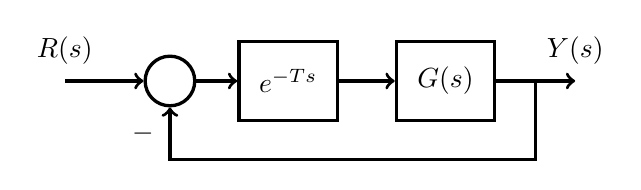
\begin{tikzpicture}[very thick,
sysblock/.style={draw,rectangle,inner sep=6pt,minimum width=1.25cm,minimum height=1.0cm,very thick},
summer/.style={circle,draw,very thick}]
\draw (0,0) node[summer] (sum) {\rule{10pt}{0pt}};
\draw (1.5,0) node[sysblock] (C) {$e^{-Ts}$};
\draw (3.5,0) node[sysblock] (G) {$G(s)$};
\draw[<-] (sum.180) -- ++(-1,0) node[above=2pt] {$R(s)$};
\draw[->] (sum.0) -- (C.180);
\draw[->] (C.0) -- (G.180);
\draw[->] (G.0) -- ++(0.5,0) |- ++(0,-1)  -| (sum.-90) node[below left=2pt] {$-$};
\draw[->] (G.0) ++(0.5,0) -- ++(0.5,0) node[above=2pt] {$Y(s)$};
\end{tikzpicture}

\noindent The Bode plot of $G(s)$ is shown below. 

%\includegraphics[width=5.5in]{.\Problem08bode.pdf}
\includegraphics[width=5.5in]{\mainfolder/LectureNotes/\lecturefolder/HomeworkProblems/Problem08/Problem08bode.pdf}


\begin{enumerate}[(a)]
\item If the time delay $T = 0 s$, what are the gain and phase margins?
\item What is the maximum time delay the closed-loop system can tolerate before going unstable? You may leave your answer as a function of $\pi$.
\end{enumerate}